\documentclass{article}

\usepackage[hidelinks]{hyperref}

\usepackage{tikz}
\usetikzlibrary{matrix,chains,positioning,decorations.pathreplacing,arrows}

\usepackage[color=cyan]{todonotes}

\usepackage{minted}
\usemintedstyle{colorful}

\usepackage{graphicx}
\graphicspath{{./images/}}

\addtolength{\oddsidemargin}{-.875in}
\addtolength{\evensidemargin}{-.875in}
\addtolength{\textwidth}{1.75in}

\addtolength{\topmargin}{-.875in}
\addtolength{\textheight}{1.75in}

\bibliographystyle{plain}

\begin{document}

\title{An Application of Deep Neural Networks to Programming Language Classification}
\author{Erik Boesen, Candidate gsg256}
\maketitle

\begin{abstract}
We assess the extent to which artificial neural networks can be used to distinguish between programming languages. We use a deep neural network to achieve a success rate of 84.00\% at distinguishing between 8 different programming languages following supervised training.
\end{abstract}

\section{Introduction}
In this research we examine the the popular machine learning technique of neural networking, specifically within the area of deep learning. In order to illustrate this technology, we outline and implement a neural network which learns to differentiate between the world's 10 most commonly used programming languages.\footnote{According to the TIOBE Index \cite{tiobe}, a popular index tracking the prevalence of programming languages as measured by search engine queries. The top 10 languages according to the May 2018 iteration of the Index are Java, C, C++, Python, C\#, Visual Basic .NET, PHP, JavaScript, SQL, and Ruby. However, our repository of training data, RosettaCode, has a limited amount of SQL code available. In order to balance the training process out, we have exchanged SQL for R, which comes in at \#11 on the TIOBE index.} The learning techniques used are generalizable to any selection of languages, as the neural network we design can be trained with any inputs and has no intrinsic understanding of specific syntactic features of any language. In order to perform identification, the network will be fed data on individual blocks of code, and will gradually adjust its weights and biases in order to ``learn'' the attributes of each language without being explicitly instructed. Having learned to distinguish between languages, it will be able to perform this task without further feedback, exhibiting well the manner in which computers are able to be trained through Machine Learning techniques.

\subsection{A general overview of neural networks}
\subsubsection{Why use a Neural Network?}
For many problems within computer science, a programmer attempts to find the function $f(x)$ mapping one or more variables to an ouput. For some problems, programmers are able to write trivial code performing human-readable mathematical operations. However, consider problems as complex as recognizing the human language being spoken in an audio file. The difficulty of writing static code to perform this task would be monumental. This sort of problem is where machine learning shines \cite{10algos}.

Machine learning refers to a broad set of techniques wherein computers, through various techniques and mathematical constructs, are able to interpret data, find patterns, and learn to make decisions sans excessive human interference \cite{sasml}. Machine Learning techniques are useful when a large and diverse set of data must be processed (often categorized), but when writing explicit code to make distinctions between data points would be impractical. Another classic example of the utility of Machine Learning techniques is the challenge of image recognition. When identifying objects in an image, as in \cite{hinton12}, an unimaginably large amount of data needs to be taken into account for each input. Without machine learning, a programmer would need to write a prohibitively large amount of esoteric code. If such a task could even be accomplished, the excessive number of edge cases for which this poor programmer would need to account would make such an application unimaginably laborious to develop. With the benefit of machine learning, however, a programmer need only instruct his or her computer to look through already-identified images, identifying the qualities of each object class and learning to make distinctions completely on its own.

Though there exist simpler machine learning techniques, such as the classic linear regression or the K Nearest Neighbors algorithm, these strategies have trouble making decisions in so many dimensions of input as demonstrated in \cite{knnic}. For such problems, neural networks are often used and are the subject of much study. Though the notion of a neural network was first proposed in 1958 \cite{rosenblatt58}, this technique has recently experienced a resurgence of popularity. Machine learning techniques based on neural networks including deep learning \cite{mitdeeplearning} and recurrent neural networks \cite{recurrentsurvey} have recently been applied to diverse problems, including achieving victory over a human in the age-old game of Go \cite{go1}\cite{go2}, differentiating between multiple thouands of different image classes \cite{hinton12}, and even recognizing verbal speech \cite{rnnspoken}.

\subsubsection{Structure of a Network}
Simply put, neural networks make tasks like the aforementioned easier by taking cues from neurobiology and simulating how a real brain adapts and makes decisions. In the brains of humans and other animals, many neurons are joined together. These neurons themselves simply take electrical input, adjust it, and pass it along to the next neuron. Biological brains readjust the behavior of their individual constituent neurons, and in doing so are able to perform the process of learning.

Though this is an oversimplification of the actual biological processes of learning and neuroplasticity, it may be a helpful metaphor to understand the function of an artificial neural network.

A neural network is composed of several groups (``layers'') of ``neurons.'' Much like in a biological brain, these neurons take input from the previous layer's neurons and use that input to make a decision on what information to pass on to the following neuron. The process performed by each neuron during decision making is relatively simple and is thus easier to think about outside the context of a larger network. First, the neuron sums the output values $\xi$ of all neurons from which it recieves input, multiplying each input value by a ``weight'' $\omega$. These weights, having been calculated during the process of training the network, essentially represent the importance of the input neuron for making the particular decision on which the network is working. To this weighted sum is added a static or dynamic ``bias,'' which can create a threshold for the neuron to fire. This result then pass through an activation function, which brings the output into a regular range such as $(0, 1)$ or $(-1, 1)$.\footnote{There exist some activation functions, such as the modern ReLU or leaky ReLU, which do not place such a limit on their output \cite{activationfunctions}. These are beyond the scope of discussion for now, however interested readers are invited to read further on this particular topic.} There exist many different activation functions, however, in this investigation we use the common $\sigma$ (``sigmoid'') function, which limits our neuron's output to $(0, 1)$:
$$\sigma(x)=\frac{1}{1+e^{-x}}$$
Hence, you may think of the neuron output $\mathcal{O}$ thus:
$$\mathcal{O}=\sigma(\sum_n[w_{n}\xi_{n}]+b)$$
After the activation function is applied, the returned value is given as the neuron's output, and the process is repeated, using that output as the input for successive neurons. A single neuron, hence, might be visualized as follows:\footnote{Original graphic rendering code sourced from \cite{neurondiagrams}.}

\begin{center}
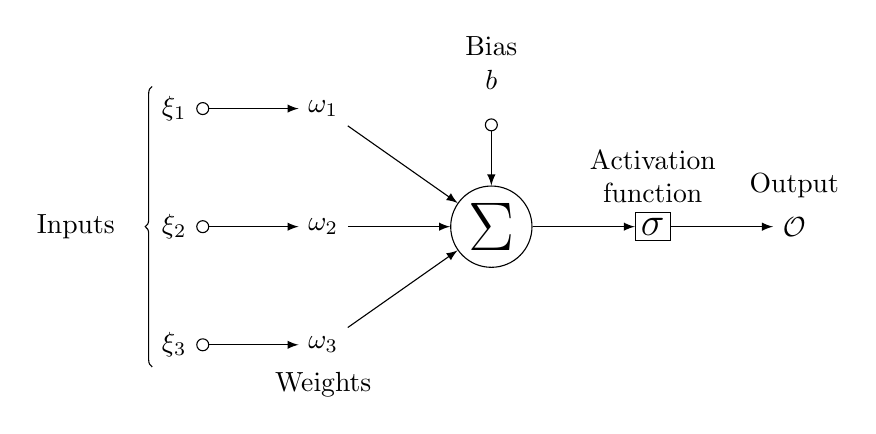
\begin{tikzpicture}[
init/.style={draw, circle, inner sep=2pt, font=\Huge, join = by -latex},
squa/.style={draw, inner sep=2pt, font=\Large, join = by -latex},
start chain=2,node distance=13mm
]
\node[on chain=2] (x2) {$\xi_2$};
\node[on chain=2, join=by o-latex] {$\omega_2$};
\node[on chain=2, init] (sigma) {$\displaystyle\Sigma$};
\node[on chain=2, squa,label=above:{\parbox{2cm}{\centering Activation \\ function}}] {$\sigma$};
\node[on chain=2, label=above:Output,join=by -latex] {$\mathcal{O}$};
\begin{scope}[start chain=1]
  \node[on chain=1] at (0,1.5cm) (x1) {$\xi_1$};
  \node[on chain=1, join=by o-latex] (w1) {$\omega_1$};
\end{scope}
\begin{scope}[start chain=3]
  \node[on chain=3] at (0,-1.5cm) (x3) {$\xi_3$};
  \node[on chain=3, label=below:Weights, join=by o-latex] (w3) {$\omega_3$};
\end{scope}
\node[label=above:\parbox{2cm}{\centering Bias \\ $b$}] at (sigma|-w1) (b) {};

\draw[-latex] (w1) -- (sigma);
\draw[-latex] (w3) -- (sigma);
\draw[o-latex] (b) -- (sigma);

\draw[decorate,decoration={brace,mirror}] (x1.north west) -- node[left=10pt] {Inputs} (x3.south west);
\end{tikzpicture}
\end{center}

Understanding now the basic logic behind individual neurons, we turn to the the architecture of a full neural network. The most basic network format, known frequently as ``feed forward,'' contains three types of layers, each of which is a vector of neurons, each taking input from every neuron in the previous layer without interacting with the rest of the layer.
\begin{itemize}
\item{The first layer is the \textbf{input layer}. Input data for the network's decision making process, which must be of a consistent size, is fed directly into this layer, and the number of neurons typically is the same as the number of possible input values.}
\item{Following the input layer comes at least one \textbf{hidden layer}. Networks with more than one hidden layer are typically used for more complex problems, and are referred to as ``deep neural networks.'' The output values of the neurons in these layers are not necessarily returned to a user, rather, they are passed on to the following layer, which can be the output layer or another hidden layer.}
\item{Neurons in the \textbf{output layer} return the output of the neural network. Note that traditionally, an activation function is implemented here as well, so basic feed forward networks are generally capable only of outputting a value in the range of the chosen activation function. In some problems, there will be only one output neuron giving a probability, from $0$ to $1$, of some relevant data point $f(x)$ being true. Classification networks designed to distinguish between several categories of input typically use multiple neurons in the output layer giving the probabilities that the input fits into each group.}
\end{itemize}

It may be useful to understand the structure of a neural network through a graphical example \cite{neurondiagrams}, where $\xi_n$ represents a scalar input to the network and $\mathcal{O}$ its single output.
\begin{center}
\begin{tikzpicture}[
plain/.style={draw=none, fill=none},
net/.style={matrix of nodes, nodes={draw, circle, inner sep=8pt}, nodes in empty cells, column sep=2cm, row sep=1pt}, >=latex
]
\matrix[net] (mat)
{
|[plain]| \parbox{1.3cm}{\centering Input\\layer} & |[plain]| \parbox{1.3cm}{\centering Hidden\\layer} & |[plain]| \parbox{1.3cm}{\centering Output\\layer} \\
& |[plain]| \\
|[plain]| & \\
& |[plain]| \\
  |[plain]| & |[plain]| \\
& & \\
  |[plain]| & |[plain]| \\
& |[plain]| \\
  |[plain]| & \\
& |[plain]| \\    };
\foreach \ai [count=\mi ]in {2,4,...,10}
% TODO: Figure out how to actually use TIKZ
\node[circle,1.2cm] (mat-\ai-1) at (-4.25,-1.68*\mi+3.9) {$\xi_\mi$} +(0,0);

\foreach \ai in {2,4,...,10}
{\foreach \aii in {3,6,9}
  \draw[->] (mat-\ai-1) -- (mat-\aii-2);
}
\foreach \ai in {3,6,9}
  \draw[->] (mat-\ai-2) -- (mat-6-3);
  \draw[->] (mat-6-3) -- node[above] {$\mathcal{O}$} +(2cm,0);
\end{tikzpicture}
\end{center}

\subsection{Backpropogation}
A central component of neural network training is the process of backpropogation. In very general terms, backpropogation is the process of determining the error of the network, or the difference between output the network delivers and desired output, and subsequently going backward through the network and adjusting neuron weights and biases accordingly.

To calculate error for an individual output neuron, the process is quite simple: we need only to find the difference between the neuron output $\omega_n$ and the known target value $t_n$.
$$E_n=t_n-\mathcal{O}_n$$
For networks with multiple output neurons, we can expand this function to find the total error of the network during one epoch (training iteration) as follows. This equation is frequently referred to as the ``cost function.'' \cite{mediummlbasics}
$$C=\frac{1}{2}\sum_n(t_n-\mathcal{O}_n)^2$$
In the context of popular neuroscience (originally in \cite{neuronsfire}), the adage that ``neurons which fire together, wire together'' is frequently repeated. This concept persists in artificial neural networks as well as natural. Through backpropogation we can determine which weights and biases to increase or decrease and to what extent to do so. Through backpropogation, we recursively readjust weights proportionally to their influence on output so as to achieve a more accurate result.

The essence of backpropogation lies in calculating $\frac{\partial{C}}{\partial{\omega}}$ for each network weight $\omega$ and $\frac{\partial{C}}{\partial{b}}$ for each network bias $b$. We need to know the extent to which shifts in each synapse weight and layer bias affects the final amount of error, so that we can adjust those weights and biases in order to train the network toward better accuracy.

Let us first derive the backpropogation algorithm \cite{derivebackprop}. Given the sigmoid activation function:
$$\sigma(x)=\frac{1}{1+e^-x}$$
We can derive:
$$\sigma'(x)=\frac{e^-x}{(1+e^-x)^2}=\frac{(1+e^-x)-1}{(1+e^-x)^2}=\frac{1+e^-x}{(1+e^-x)^2}-\left(\frac{1}{1+e^-x}\right)^2=\sigma(x)-\sigma(x)^2=\sigma(x)(1-\sigma(x))$$

Now, recall that we need to find, for each weight $\omega$, $\frac{\partial{C}}{\partial{\omega}}$. For the sake of simplicity, we will need to split this partial derivative into a series of the same. This expansion requires us to make use of calculus' chain rule.
$$\frac{\partial{C}}{\partial{\omega}}=\frac{ \partial{C} }{ \partial{\mathcal{O}} }
                                        \frac{ \partial{\mathcal{O}} }{ \partial{z} }
                                         \frac{ \partial{z} }{ \partial{\omega} }$$

Where $z$ represents the weighted sum, plus the bias, of the neuron's inputs before application of the activation function.

Now we must compute an actual equation to find $\frac{\partial{C}}{\partial{\omega_h}}$. This is relatively simple as we know most of the expressions we must differentiate to form the components of the above expansion.

$$\frac{\partial{C}}{\partial{\mathcal{O}}}(\mathcal{O}-t)^2=2(\mathcal{O}-t)$$
$$\frac{\partial{\mathcal{O}}}{\partial{z}}\sigma(z)=\sigma'(z)=\sigma(z)(1-\sigma(z))$$
$$\frac{\partial{z}}{\partial{\omega}}(\omega\mathcal{O}_h+b)=\mathcal{O}_h$$

Where $t$ is the target output of the neuron, provided from an outside source during training.

If we combine these three constituent partial derivatives, we can find $\frac{\partial{C}}{\partial{\omega_h}}$ as we desire:
$$\frac{\partial{C}}{\partial{\omega}}=2(\mathcal{O}-t)\sigma(z)(1-\sigma(z))\mathcal{O}_h$$

The rate of change of the cost function relative to a bias term, $\frac{\partial{C}}{\partial{b}}$, can be computed in a similar manner, simply trading $\frac{\partial{z}}{\partial{\omega}}$ in return for $\frac{\partial{z}}{\partial{b}}$.

$$\frac{\partial{z}}{\partial{b}}(\omega\mathcal{O}_h+b)=1$$
$$\frac{\partial{C}}{\partial{b}}=\sigma(z)(1-\sigma(z))\mathcal{O}_h$$

\todo{FINISH}
During backpropogation, these derivatives can be used in the ``gradient descent algorithm'' to move downhill in $n$ dimensions toward a local minimum of the cost function, bringing the network closer to correctness.

\section{Programming Language Identification}
\subsection{Motivations}
There exists a great deal of academic literature regarding the use of neural network techniques to recognize and distinguish between natural languages, through media including speech \cite{rnnspoken}\cite{dcrnnspoken}, handwriting \cite{handwritingex}, and typed text \cite{langidnn}\cite{langidstanford}. However, very little research has been performed on the recognition of programming languages. We note several possible causes of this deficit of scholarship:
\begin{itemize}
    \item{Programming languages are, almost without exception, input directly into a computer through keyboard I/O or automatic generation (metaprogramming). There are almost no occasions where code must be input orally or through handwriting, and, in the latter case, roughly identical technologies can be used as with traditional language writing. So, the need for research on nontraditional means of code input, such as through writing on paper, optical character recognition, or oral dictation, is infrequent and may overlap with existing research on natural language processing.}
    \item{Code is generally stored in files with extensions, enabling simple recognition: no machine learning required. Files whose names end in \texttt{.c} obviously contain C code, and those with \texttt{.py} extensions can be reasonably assumed to contain Python code. Some software, such as the Atom text editor and the website GitHub \cite{githubid}, rely predominantly upon the extension of a file to determine the language of its contents. This clearly is not possible with traditional written language, which only in defined cases comes packaged in files whose names give computationally valueable information about the chosen tongue.}
    \item{Even when files lack an extension, there often exist indicators of language used at the beginning or within the body of a code document. Code written in the markup language \cite{htmlnotproglang} HTML generally begins with \mintinline{html}{<!DOCTYPE html>}. Documents using interpreted languages such as Shell (and derivatives), Python, Ruby, or Perl, may begin with a ``shebang,'' such as \mintinline{bash}{#!/usr/bin/env bash}, specifically providing the system with a path to the interpreter even if no file extension is included \cite{shebang}. Within the document, further programatic determinations can be made, for example, any file at any point containing \mintinline{php}{<?php} is almost certainly written in PHP. However, these markers are not always present.}
\end{itemize}
While it's clearly not always necessary to recognize a language by its raw syntax, there are some occasions in which such a task may be advantageous to perform. Some examples:
\begin{itemize}
  \item{It is possible for a user to write an interpreted script, such as one in an interpreted derivative of Shell, without using a shebang or otherwise manually specifying the language of interpretation. In this case, the program loader would generally run the script automatically using the shell from which execution was performed \cite{shebang}. However, a text editor in which the program is being edited may lack practical means of determining which language is being used, giving the absence of connection to the running shell.}
  \item{Some file types/extensions are used by multiple languages. For example:
  \begin{itemize}
    \item{\texttt{.sh} is sometimes used for many different variations of shell script, even though some of those varieties (like \texttt{tcsh}) are syntatically incompatible.}
    \item{The extension \texttt{.h} is used for header files in C, C++, Objective-C, Objective-C++, and other C-like languages.\footnote{Note that the extensions \texttt{.hpp} and \texttt{.hh} exist for C++ headers. However, this standard is inconsistently applied, and \texttt{.h} is commonly used for all these languages. Additionally, there are still conflicts evident with Objective-C and Objective-C++. More information can be found regarding the relevant standards and their implementation at \cite{atomh}.}}
    \item{\todo{Start this with a sentence describing these sorts of events}Some languages, like Ruby and Python, are used within HTML templates in some web frameworks. Flask \cite{flaskwebsite}, a Python web app microframework, uses the Jinja2 templating system to perform programatic logic within an HTML file, which maintains its traditional \texttt{.html} file extension.}
  \end{itemize}
  In these instances, it's impossible to tell from a file's extension what language is being used: indeed, an educated guess may even be straightforwardly wrong.}
  \item{During programming competitions or other instances where code is written directly into an online input field, it may be useful to automatically determine the language in which a participant is writing their solution to a problem, rather than forcing the user to input their choice of language manually.}
\end{itemize}
For human observers with experience in programming, recognizing the language of a piece of code is a trivial task. As is the case with countless machine learning problems, to do so in an automated fashion is more difficult. Here we will use a feed-forward neural network. There exists no scientific literature on this topic. The only evident instance we could locate of such a task being completed is a single blog post from 2016 \cite{proglangidmedium}.

We will take several cues from preceding research on recognition of textual language. While the task of programming language syntax recognition is not identical to identification of natural human languages, we can borrow some ideas from such research.

\section{Implementation}
In order to illustrate the concepts above described, we implement a simple feed-forward neural network to learn from training samples.

\subsection{Training Data}
To train our network, we use dumps of code in each programming language obtained from the ``programming chrestomathy'' website RosettaCode \cite{rosettacode}. The website provides diverse solutions to a wide variety of programming problems in hundreds of different languages. Because it has such varied code written in the languages we've selected from a diverse group of programmers written with many different styles, it is a perfect source of training data in the languages we select. Training on too-homogenous data could negatively impact our network's ability to process code samples unlike those it has seen before. Code used to download and build training and testing data may be found in  \hyperref[sec:appendix_a]{Appendix A}.
\subsection{Platform}
The network was implemented in the Python programming language using the library Keras, which abstracts neural network creation \cite{keras}.

Basic feed-forward neural networks are unable to handle input vectors of variable sizes. Because of this, it's not possible for us to input whole files of code at once and recieve a result. We must instead find a way of breaking up code files into bite-sized sections to use as training examples.

Most research on natural language recognition, including \cite{langidstanford}, use $n$-grams of raw or processed text as input vectors. $n$-grams are perfect for such an application, as they allow the network to learn about patterns evident in word structure and alphabet choice and to standardize input vectors in a simplistic manner. However, for the problem of programming language classification, $n$-grams may not be the best solution. In initial trials using $4$- and $8$-grams of characters, the network failed to correctly choose the language of most training samples due to the ambiguity of most $n$-grams.

From investigation of the samples where incorrect predictions were made, we found that most contained simple English text, written in in-code ``comments,'' or natural-language explanations of code written directly into the code document.

Such an outcome is difficult to avoid when separating by $n$-grams. Short of artificially cleaning comments from source files in training and evaluation of new data, our network may become confused by excessive amounts of plain natural-language text which do not vary between programming languages.

Instead, we will create input vectors by reading in $1000$-character strings of code, and, rather than directly passing in character values, calculating character frequency relative to the total number of counted characters, and passing in this data as an input vector. Ideally, the network will recognize the relative unimportance of those characters irrelevant to the identity of a piece of code, such as alphanumeric characters, while relying more on indicators like semicolons or brackets.

From close observation of relative letter frequencies in our training data, some trends are notable:
\begin{center}
    \makebox[\textwidth]{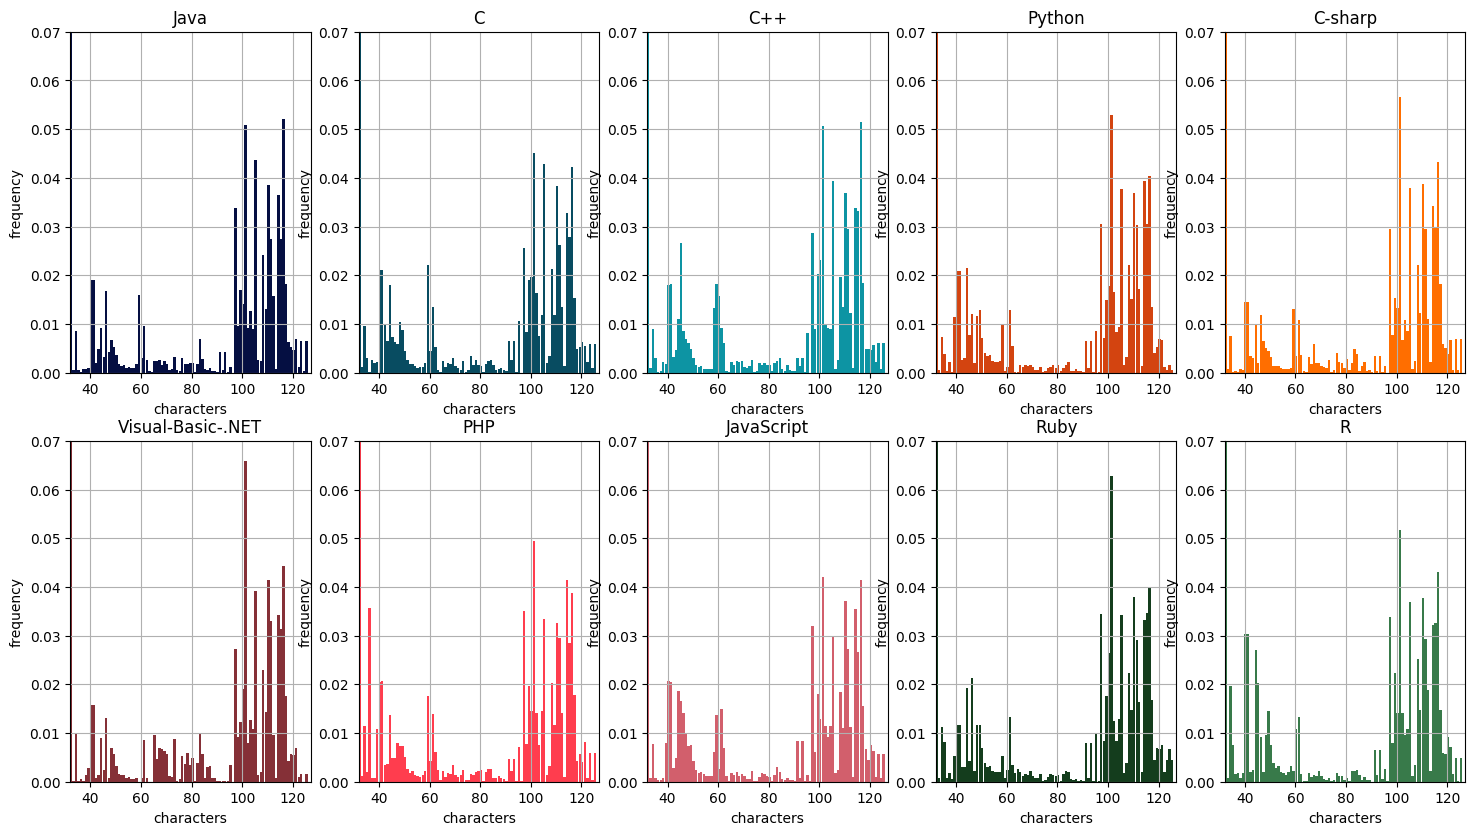
\includegraphics[width=\textwidth]{frequencies}}
\end{center}

To build our network, we chain together four layers. The first (input) layer, with 94 total neurons. This number is based off the range of ASCII characters we wish our to regard in making its decisions \cite{asciitable}. Characters before point 32 (Space) are used for various purposes such as connection maintenance and terminal life control and are not useful for identification of language. Range 32-126 inclusive contains punctuation, Western Arabic digits, and both uppercase and lowercase letters. While characters outside this range may appear in code from time to time, they are unlikely to be significant to the identity of a code document, and as such will be ignored.

\begin{center}
    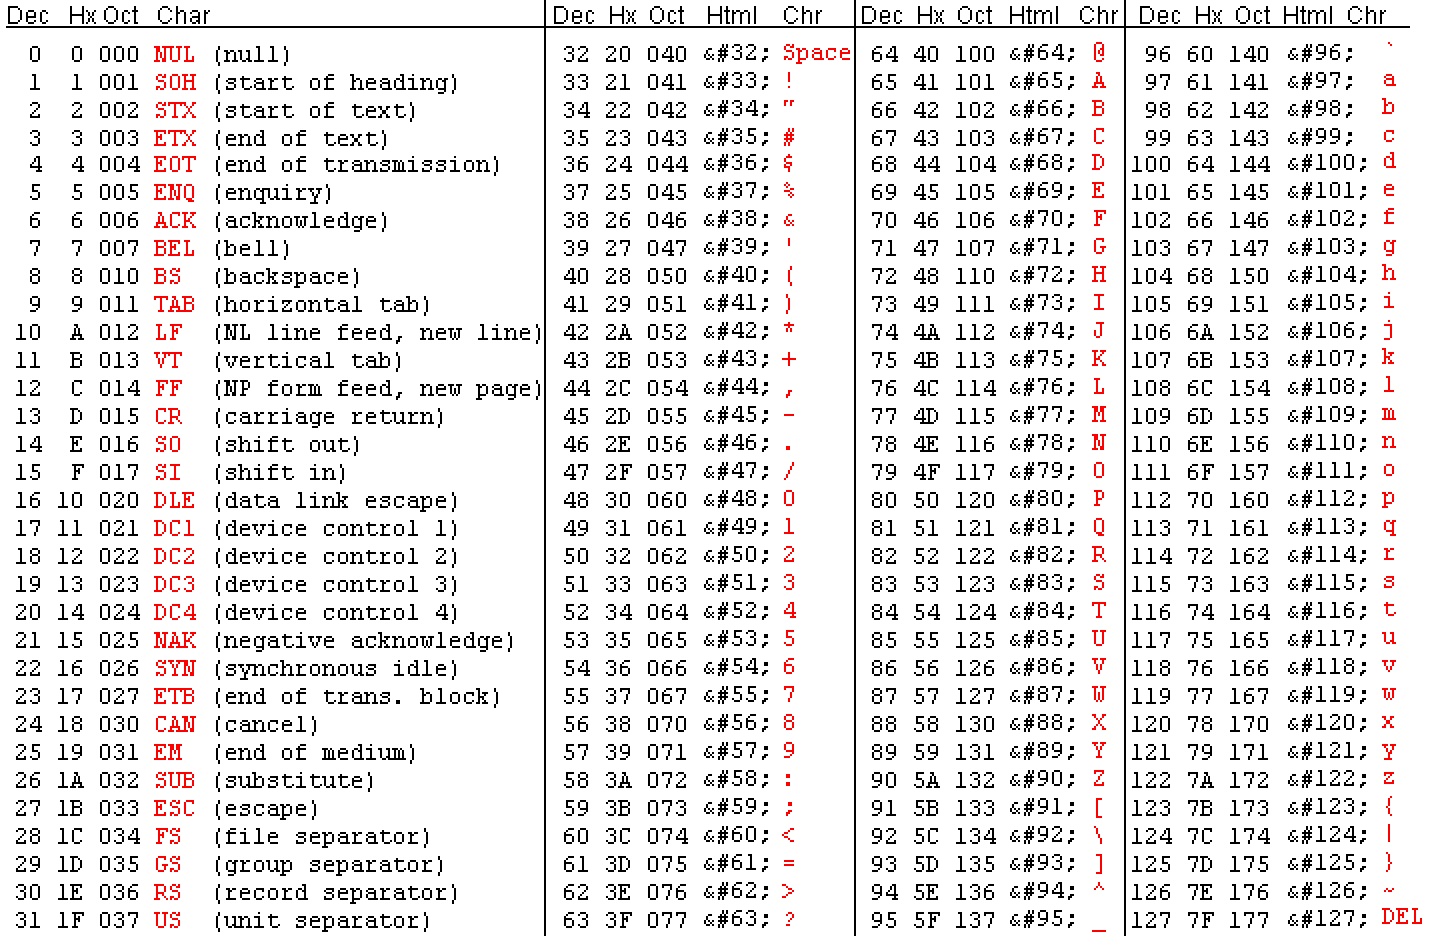
\includegraphics{asciitable}
\end{center}

Each character in this relevant range is counted within each training example of $1000$ characters. Input neurons recieve a number in the range $[0,1]$ and use this data in forward propogation.

The network contains two hidden layers of size 48 and 24 neurons. These sizes are relatively arbitrary; training would likely still succeed with other hidden layer sizes.\todo{Explain this better?}

The output layer will contain 10 output neurons, expressing a probability ($[0..1]$) that the code is written in each of the 10 languages.

\section{Results}
Though our network's predictions are not flawless, the network structure we propose is able to make predictions with an accuracy between 80 and 90\% depending on the layout of the data provided. To be specific, the network attained an accuracy of 84.00\%.

We can visualize the evolution of our network throughout the training process by looking to its accuracy and loss (cost function) during the training process:

\begin{center}
    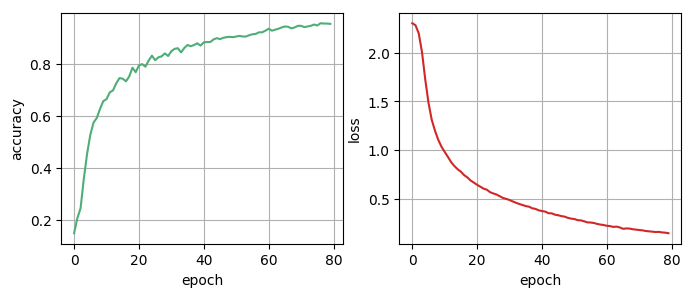
\includegraphics{history}
\end{center}

As any other network would, Random guessing would yield an accuracy around 10\%, so this accuracy is impressive.

\section{Future questions and improvements}
The network certainly is far from perfect, and future research is needed to refine the techniques expressed above. Concretely, a few opportunities for improvement are evident.
\begin{itemize}
  \item{In order to simplify the process of reading data, we concatenate all training samples for each language into one file. This may lead to unpredictable behavior as, for example, the program might gain the impression that an $n$-gram such as
  \begin{minted}{c}
// ...
    return 0;
}
#include <stdio.h>
// ...
  \end{minted}
  is normal.\footnote{C/C++'s \texttt{\#include} statement seldom comes anywhere but the beginning of files.} This is not likely to interfere substantially with the identification process, however, the abnormal way in which we group the files is a point worthy of reflection and possible change.}
  \item{In addition to the weights on connections, biases can be configured to }

\end{itemize}


\section{Appendices}

\label{sec:appendix_a}
\subsection{Appendix A: Scripts for building training data}
Training and testing data for our neural network is retrieved from \url{http://rosettacode.org/}, a website which aggregates solutions to a wide variety of programming problems. This makes it an ideal source of diverse code using varied syntax.

Data is retrieved from an index on the code-sharing website GitHub\cite{rosettacodegh} using the script \texttt{download.sh}:
\inputminted{bash}{code/data/download.sh}

\label{sec:appendix_b}
\subsection{Appendix B: Compilation and System Constants}
All C++ code was compiled on an Amazon Web Services EC2 Instance running SUSE Linux Enterprise Server 12 (x86\_64). The package \texttt{gcc-c++} was installed on the system, and g++ 7.2.1 20171005 was used for compilation. Some testing was also performed on Mac OS X 10.11.6.

\label{sec:appendix_c}
\subsection{Appendix C: Reader code}
We use a simple header \texttt{reader.hpp} to define the class and methods of our reader:
\inputminted{cpp}{code/reader.hpp}
Then, we implement all methods in \texttt{reader.cpp}:
\inputminted{cpp}{code/reader.cpp}
\todo{This code doesn't quite do everything we need}

The following \texttt{Makefile} was used in all instances:
\inputminted{makefile}{code/Makefile}

\section{Acknowledgements}
I would like to thank Mr. William Snyder for serving as the advisor for this Extended Essay. Ms. Jamie Sample was the Extended Essay Coordinator for the GMHS IB students within the Class of 2019. I'd also like to extend my regards to James Weichert for fighting through his essay on a similar topic alongside me and for pointing me toward numerous terrific resources for grasping the mathematical technique behind neural networks. Finally, I'd like to give my most heartfelt gratitude to Stack Overflow, without which I would never have reached the point of attempting a Computer Science EE in the first place.

\bibliography{research}

\end{document}
